%!TEX root = ../masters_thesis.tex

\chapter{Concept} % (fold)
\label{cha:concept}

domain: development of countries in time and space

usable User Interface for both navigation and editing
-> problem: all interfaces are trés horrible!

research questions --> HGIS <-- development of system
  historians /                           ME
  geographers
(+) open source, direct manipulation, easy sharing and collaboration



% ==============================================================================
\section{Hivent-Based Spatio-Temporal Data Model} % (fold)
\label{sec:hivent_based_spatio_temporal_data_model}

no perfect data model possible, because a model is just an incomplete abstraction of the real world

estd for vector graphics

3 domain model
identity: formal name of an entity

history graph model without changing state: active, inactive

simplification: just active / inactive, normal / contested + level of certainty

Hivent-Based Three-Domain Spatio-Temporal History Graph Data Model for Vector Geometry
... or in short: HBTDSTHGDMVG

no transaction time, only valid / event time
only world time is regarded, not database time.


interior borders of countries, which are straight lines between manually defined border points.
=> vector model

A main problem is to maintain the integrity of the spatial topology when a new change gets inserted not at the end of the list. A simple example shows that problem: Given geo-object $X$ is part of the inital base configuration at change $t_b$. At a later change, e.g. $t_y$ $X$ gets replaced by object $Y$. If a new change that updates $X$ to $X'$ gets inserted before at time point $t_x < t_y$, then $t_y$ is not integer anymore, because object $X$ does not exist. That is why on insertion of a change, all succeeding changes have to be tested for integrity and it might be necessary to update later changes.

% \begin{figure}[ht]
%   \centering
%   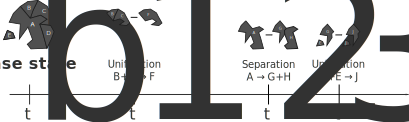
\includegraphics[width=0.8\textwidth]{graphics/basics/stdm/event-based_spatio-temporal_data_model}
%   \caption{The Event-Based Spatio-Temporal Data Model}
%   \label{fig:event-based_spatio-temporal_data_model}


\paragraph{possible extension} % (fold)
\label{par:possible_extension}

% paragraph possible_extension (end)

-> the whole earth is 100\% covered by spatial objects (full topology)
  countries, debated territories, unknown land, water
  Newtons concept of absolute space?



% ==============================================================================
\subsection{Hivent} % (fold)
\label{sub:hivent}

event which is in itself or whose outcome is historically significant (subjective) or with

  WHAT? significant happening
  WHO? different actors
  WHEN? one point in time
  WHERE? mostly also point in space, sometimes different from area that event affects
  WHY? because

models historically significant happenings with a focus on those who influence the geopolitical history of countries.

In modern history, geopolitical changes of countries are manifested mostly in historical treaties which are the result of a conference or any other gathering of representatives of stakeholders of that initiated change. Since each of those treaties is signed on one particular day, in one particular place and has one particular name, the ~\texttt{Hivent}~ model seems appropriate.

However, the first question arises regarding the relevance of the location: While the exact position of the battlefield of Verdun or the place where John F. Kennedy was assassinated might very relevant to the event itself, the location of a governmental bill, a declaration of independence or a border convention might not play an important role and usually happens in a representative place, e.g. the parliament or the office of a president. In a lot of cases, it is much more important which territories an event actually influences instead of where it happened.

significant happening in time and space
incluencing others
central element in event based STDM

store Hivents in DoublyLinkedList

% subsection hivent (end)


% ==============================================================================
\subsection{Area} % (fold)
\label{sub:area}

model the main entity of the domain: historical or current countries. An ~\texttt{Area}~ represents one identical country, consisting at each time point of its existance of exactly one ~\texttt{AreaName}~ and one ~\texttt{AreaTerritory}. The model seems appropriate since the name and the territory of an area are exactly the two properties that are part of the domain.

abstract: area

  defined by borders
  hierarchical structure

countries with enclaves or islands are not topologically equivalent.

country borders
  coastlines
  interior
  disputed territories
    situation: n fully recognized countries and m non or partially recognized entities claim sovereignty over 1 territory
    territory is surrounded by disputed border
    question: does this disputed area claim sovereignty?
    \footnote \url{http://www.economist.com/blogs/economist-explains/2014/09/economist-explains-1}
  uncertain borders
    situation: n fully recognized countries commonly agree on a boundary between them, but the border is not clearly defined / fuzzy / uncertain
  states of borders
    planned
    agreed
    demarcated
    provisional
    valid
    vs. disputed

    borders: complex model: different states of boundaries: draft -> proposal -> dispute ->
    % \cite Wachowitz 1998 pp. 55


area
territory
-> geometry
--> border
-> representative point
name
-> short name
-> formal name

enclaves
exclaves



% subsection area (end)

% section hivent_based_spatio_temporal_data_model (end)


% ==============================================================================
\section{Historical Geographic Operations} % (fold)
\label{sec:historical_geographic_operations}

CRE
UNI
INC
SEP
SEC
TCH
BCH
NCH
ICH
DES


There are topological rules rules that can be applied, e.g. two neighboring countries (polygons) share one common border (polyline). That preserves the relationship between them if their common border changes.

inclusion of universe $\Omega$:
CRE = SEC from $\Omega$
DES = INC into $\Omega$

MECE principle: Mutually Exclusive and Collectively Exhaustive

% section historical_geographic_operations (end)

% ==============================================================================
\section{HistoGlobe} % (fold)
\label{sec:histoglobe}

Application: HistoGlobe
A distributed \emph{Web Information System}, consists of a remote server side, on which the storage and management of the actual data happens, and the client side on which the user communicates with the system. It hosts the user interface that is rendered in a Web browser.

map for spatial domain (x, y)
timeline for temporal domain (t)
-> 3D system

describe the components of the HG explicitally

ancestors successors
layers of administrative units
open to extension for additional attribute data (e.g. statistics)

requirements
  geographical knowledge
  contextualize / intersect historical sources
  accept imprecision
  prevent illusion of certainty

% ------------------------------------------------------------------------------
\subsection{System Architecture} % (fold)
\label{sub:system_architecture}

The system developed in this thesis is Web-based. That means, there is a \emph{client}, a Web browser, and a remote Web \emph{server} with a database and a middleware. The Web browser hosts the applications user interface. If the user interacts with a tool the client sends a request to the Web server for new data. The middleware checks the request and queries the necessary data from the database. The data will be transformed and sendt back to the client. On the map and the timeline the new information will be shown.

This clear separation between the data (\emph{model}), the user interface (\emph{view}) and the middleware (\emph{controller}) follows directly from the \emph{model-view-controller pattern}: One part can be changed without interfering the other parts, e.g. if the 2D map is replaced by a 3D globe, only the view changes, but the middleware and the database can stay untouched. Likewise, the implementation of a new database technology has no consequences to the view.

% subsection system_architecture (end)


% ------------------------------------------------------------------------------
\subsection{Data Input} % (fold)
\label{sub:input}

This HGIS needs data about historical countries, their names and borders and historical events that lead to historical changes of these countries. There are a lot of free and open sources for geographic data about the current countries, their names and borders. One of the most exhaustive collections of geographic data in public domain is hosted by Natural Earth
\footnote{
  \textit{Natural Earth},
  URL: \url{http://www.naturalearthdata.com/downloads/},
  last access: 30.10.2015
}.
There is physical data (e.g. coastlines, rivers, or glacier areas) and cultural data (e.g. political borders, cities, roads, airports or timezones). OpenStreetMap also opens its database to the public
\footnote{
  \textit{Planet OSM},
  URL: \url{http://planet.openstreetmap.org/},
  last access: 30.10.2015
}.

However, data about historical countries and events are not as straightforward to aquire, because of the mostly qualitative nature of historical research (see section \ref{sub:history}). The most exhaustive free and open source of historical is the \emph{Wikipedia} and their article categories, e.g. \texttt{armistices} or \texttt{treaties}
\footnote{
  \textit{Category:Treaties},
  Wikipedia, the free encyclopedia,\\
  URL: \url{https://en.wikipedia.org/wiki/Category:Treaties},
  last access: 13.05.2016
}.
All sorts of historical events can be found, even translated into different languages. Some information is structured in information boxes, e.g. some historical treaties have a name, an image, a location, a signature and an effect date, an overview about treaty conditions and signatories. Particularily interesting for this thesis are articles about historical countries
\footnote{
  \textit{List of former sovereign states},
  Wikipedia, the free encyclopedia,
  URL: \url{https://en.wikipedia.org/wiki/List_of_former_sovereign_states},
  last access: 13.05.2016
},
because they contain the name of the country and meta information, e.g. their historical successors and predecessors. Building an open-source Historical Geographic Information System on the basis of Wikipedia would be a huge project with significant impact on the world of free and open education --- however, it would also be a big challenge: Wikipedia is incomplete, not all historical countries and events necessary to model the history of the world are available. It is also inconsistent, because not all articles about historical countries and events are structured, especially not to those who actually have an influence on a territorial change of a country, e.g. a border agreement. Retrieving, parsing and processing this information is a big challenge. Also the problem of accuracy and quality of information in the Wikipedia due to their open source nature has to be considered. Overall, using the Wikipedia as a data source for this thesis is not feasible, but is subject to further research.

% - - - - - - - - - - - - - - - - - - - - - - - - - - - - - - - - - - - - - - -
\paragraph{Historical maps} % (fold)
\label{par:historical_map}

The most problematic data to acquire is about the territories and borders of historical countries. There is no primary data source for that, so the only way to retrieve a border is to extract it from an historical map.

They also can be found on Wikipedia, or in historical map colletions, e.g. \emph{OldMapsOnline}. The project is developed ``out of a love of history and heritage of old maps'' and currently stores about 400000 historical maps
\footnote{
  \textit{Old Maps Online},
  URL: \url{http://www.oldmapsonline.org/},
  last access: 13.05.2016
}.
There are five steps to retrieve a border with points in geographic coordinates from an historical map.
\begin{enumerate}
  \item \textbf{Digitization}: If the map is on paper, it has to be scanned in the best possible quality. The result is a raster graphic.
  \item \textbf{Georeferencing}: The historical map has to fit as good possible on the reference map. This requires to manually define a set of reference points which are used to transform the map into the geographic coordinate system. This process is error-prone, especially if the projection of the historical map is not known and the map itself is not accurate
  \cite[pp. xvii]{knowles2002past}.
  The outcome is a raster graphic in which each pixel is assigned a geographic coordinate.
  \item \textbf{Preprocessing}: The raster image has to be be processed so that the desired border stands out and can be traced in the next step. This happens via greyscale conversion, thresholding or the Canny Edge Detector. This results in a monochrome graphic in which the desired border must be uninterrupted and clearly be seen.
  \item \textbf{Line detection}: By selecting a start and an end point of the border, the line gets traced automatically. This step vectorizes one particular feature, a borderline, from the raster graphic and produces a polyline in geographic coordinates.
  \item \textbf{Postprocessing}: In the last step, the polyline can be adapted: The line can be simplified to reduce unnatural artifacts and the position of border points can be manually edited. The final output of the whole process is a polyline whose points are expressed in the geographic coordinate system which can be used in the system as a border of an historic country.
\end{enumerate}

This process was developed in a preceding \emph{HiBo} project
\footnotetext{
  \textit{HiBo - semi-automatic extraction of borders from historical maps},
  Project of: B. Weber, N. K. Dankwa, K. Singh and T. Kashyappan, supervised by: Prof. Volker Rodehorst and Marcus Kossatz, Bauhaus-Universität Weimar, February 2015,
  URL: \url{https://bitbucket.org/bastian_weber/hibo},
  last access: 29.10.2015
}
(see figure \ref{fig:hibo}).

\begin{figure}[ht]
  \centering
  \begin{subfigure}{0.48\textwidth}
    \centering
    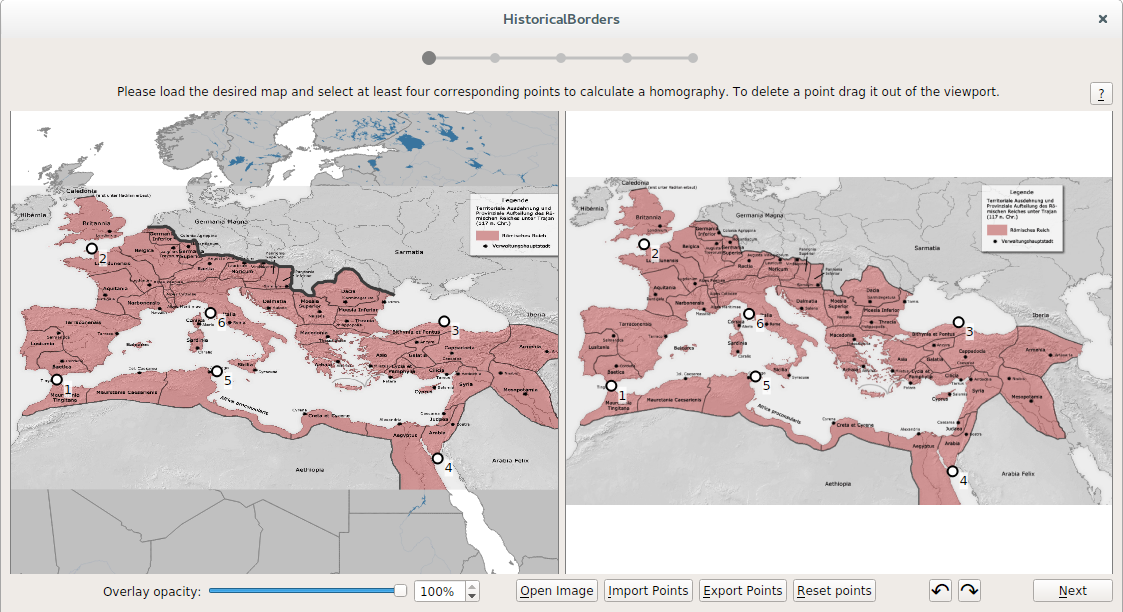
\includegraphics[width=0.95\linewidth]{graphics/basics/hibo1.png}
    \caption{Georeferencing}
  \end{subfigure}
  \begin{subfigure}{0.48\textwidth}
    \centering
    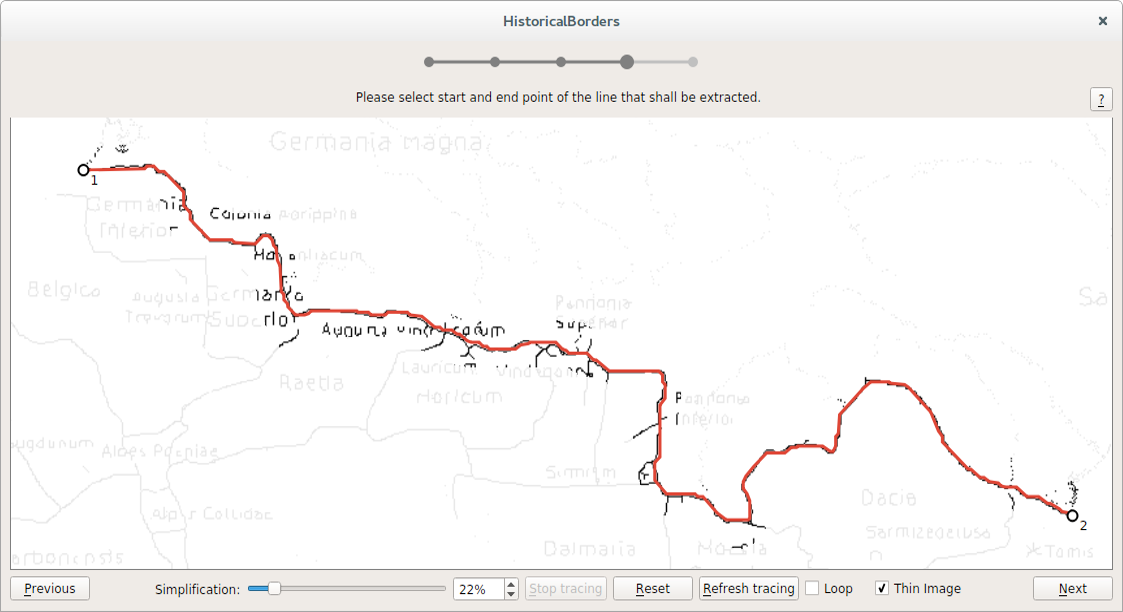
\includegraphics[width=0.95\linewidth]{graphics/basics/hibo2.png}
    \caption{Semi-automatic digitizing}
  \end{subfigure}
  \caption{Semi-automatic extraction of a border from a map of the Roman Empire \protect\footnotemark}
  \label{fig:hibo}
\end{figure}

% paragraph historical_map (end)


% - - - - - - - - - - - - - - - - - - - - - - - - - - - - - - - - - - - - - - -
\paragraph{Manual data input} % (fold)
\label{par:manual_data_input}

For the domain of this HGIS, the development of countries over time, there is no complete dataset available. Therefore, the system developed in this thesis needs to have an interface to enter historical data. The user needs to have an interface to enter information about historical events that change territories and names of historical countries. This data has to be acuired either from primary historical sources directly, or from free online sources. Next to Wikipedia, there are other collections of historical events, e.g. \emph{Correlates of War}
\footnote{
  \textit{Data Sets},
  Correlates of War,
  URL: \url{http://www.correlatesofwar.org/data-sets/folder_listing},
  last access: 13.05.2016
}
for quantitative data about international relations.
% paragraph manual_data_input (end)

% subsection data_input (end)



% ------------------------------------------------------------------------------
\subsection{Edit Mode} % (fold)
\label{sub:edit_mode}


user operations     CRE     UNI          SEP         TCH         NCH      DES
                     |      / \         /   \        /  \       /   \      |
HG operations       CRE   UNI   INC   SEP   SEC   TCH   BCH   NCH   ICH   DES

area changes        ADD   DEL*  DEL*  DEL   TCH   TCH   TCH   NCH   ADD   DEL
ADD, TCH, NCH, DES        ADD   TCH   ADD*  NCH?        TCH         DEL
                                NCH?        ADD*


geometries must be edited



% subsection edit_mode (end)

% ------------------------------------------------------------------------------
\subsection{HistoGraph} % (fold)
\label{sub:histograph}

% subsection histograph (end)

% section histoglobe (end)



% chapter concept (end)